\documentclass{article}
\usepackage{listings}
\usepackage{xcolor}
\usepackage{minted}
\usepackage{geometry}
\usepackage{float}
\usepackage{graphicx}
\usepackage{algorithm}
\usepackage{algpseudocode}
\usepackage{hyperref}
\usepackage{tabularx}
\usepackage{amsmath}

\geometry{
	textheight=9in,
	textwidth=6in,
	top=1in,
	headheight=12pt,
	headsep=25pt,
	footskip=30pt
}

\begin{document}
	
	\title{Selected Topics in Frontiers of Statistics Third Assignment}
	\author{12111620 Yixuan Ding}
	\date{\today}
	\maketitle
	\section*{Part 1}
	\subsection*{Q1}
	For question 1, networkx is utilized to generate ER network. As the question requests, the average degree of the network is 0.5. The network size is chosen to be 10000, thus the probability for connection is set to 0.00005.\\
	After generating graph, the component of the graph can be obtained, so as their sizes. Calculated the number for different sizes and gain the distribution of component size. The graph is shown below:
	\begin{figure}[H]
		\centering
		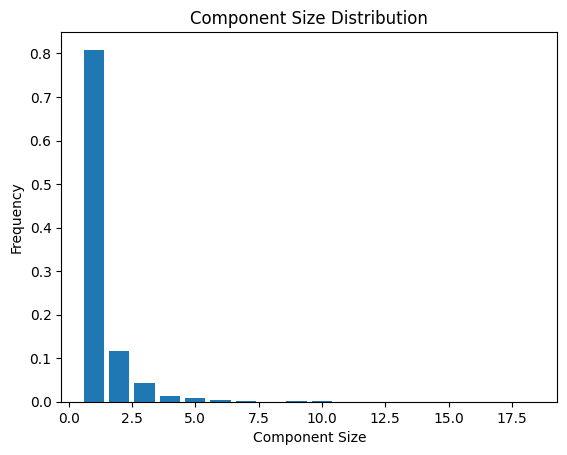
\includegraphics[scale=0.5]{P1Q1.png}
		\caption{Simulated Component Size Distribution}
	\end{figure}
	
	\subsection*{Q2}
	To calculate $P_s$ numerically, several formulation needs to be introduced:
	\begin{itemize}
		\item $G_0(x) = \sum_{k=0}^{\infty}p_k x^k$: Generating function for degree distribution.
		\item $G_1(x) = \frac{G^{\prime}_0(x)}{G^{\prime}_0(1)}$: Generating function for second layer neighbor degree distribution.
		\item $H_1(x) = x G_1(H_1(x))$: Generating function for size of component reached by choosing a random edge and following it to one of its end.
		\item $H_0(x) = xG_0(H_1(x))$: Generating function for size of component located by randomly choosing a vertex.
	\end{itemize}
	For $p_k$ of $G_0$, it can be represented by the frequency of degree in graph generated above. Then $G_1$ can be obtained by $G_0$. For the calculation of $H_1$, it is noticed that the equation is of self-consistency form, so that iteration can be utilized by setting $H_1$ to $x$ at the beginning. After calculating $H_1$, $H_0$ can be derived.
	
	Finally, $P_s$ can be derived by $$P_s = \left. \frac{1}{s!}\frac{d^s H_0}{d z^s} \right|_{z=0}$$
	The distribution of $P_s$ is shown below:
	\begin{figure}[H]
		\centering
		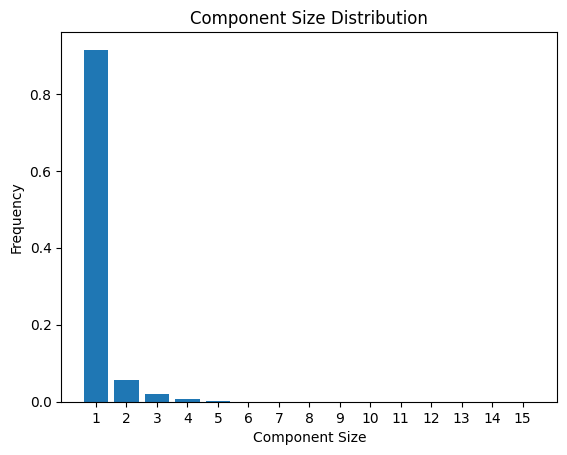
\includegraphics[scale=0.5]{P1Q2.png}
		\caption{Calculated Component Size Distribution}
	\end{figure}
	
	\subsection*{Comparison}
	The simulated component size distribution is nearly the same as the theoretic calculation of the distribution. They all have more amount of component when the size is smaller, and the number of component decays as the size growing. However, theoretically, there are more small components than simulated scenario. 
	
	\section*{Part2}
	\subsection*{Q3}
	For poisson degree distribution with average degree $<k>$, $S$ and $T$ can be calculated separately and expressed by $\langle k \rangle$.
	\[
	\left\{
	\begin{aligned}
		S &= 1 - e^{-zS} \\
		T &= \frac{1}{\langle k \rangle}
	\end{aligned}
	\right.
	\]
	Then $S = 1 - e^{-\frac{S}{T}}$, and the plot is derived:
	\begin{figure}[H]
		\centering
		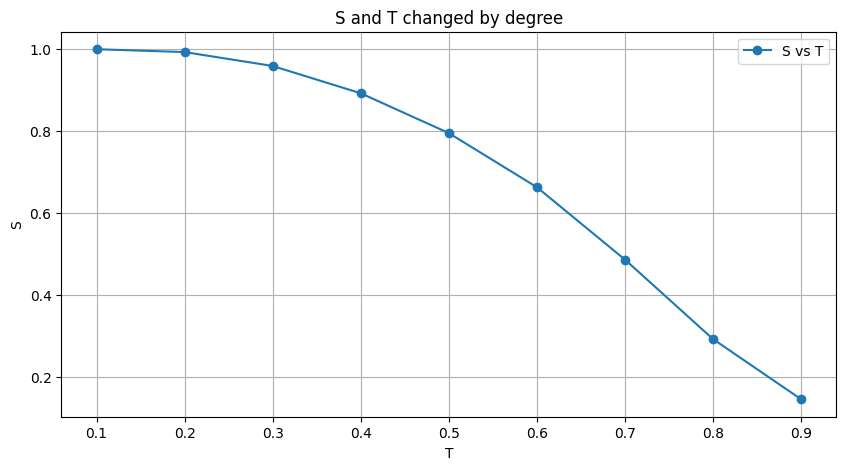
\includegraphics[scale=0.5]{P2Q3.png}
		\caption{S vs T}
	\end{figure}
	
	\subsection*{Q4}
	For power law degree distribution and $p(k) ~ k^{-2.5}$, the minimum degree and the maximum degree of the network is 2 and $\sqrt{N}$. Here N is set to 1001. First, $G_0$ is calculated by degree distribution. After that we can obtain $G_1$, $H_1$ and $H_0$ as before. Notice that:
	\[
	\left\{
	\begin{aligned}
		S &= 1- G_0(u) \, and \, u \equiv H_1(1) \\
		T &= \frac{G^{\prime}_0(1)}{G^{\prime\prime}_0(1)}
	\end{aligned}
	\right.
	\]
	By calculation:
	\[
	\left\{
	\begin{aligned}
		T &= 0.17045 \\
		S &= 0.65918
	\end{aligned}
	\right.
	\]
	
	\section*{Appendix}
	More relevant detailed information you can find in: 
	\href{https://github.com/DingYX0731/Selected-Topics-in-Frontiers-of-Statistics}{\textbf{Github Repository}}
	
	
\end{document}